% Options for packages loaded elsewhere
\PassOptionsToPackage{unicode}{hyperref}
\PassOptionsToPackage{hyphens}{url}
%
\documentclass[
  ignorenonframetext,
]{beamer}
\usepackage{pgfpages}
\setbeamertemplate{caption}[numbered]
\setbeamertemplate{caption label separator}{: }
\setbeamercolor{caption name}{fg=normal text.fg}
\beamertemplatenavigationsymbolsempty
% Prevent slide breaks in the middle of a paragraph
\widowpenalties 1 10000
\raggedbottom
\setbeamertemplate{part page}{
  \centering
  \begin{beamercolorbox}[sep=16pt,center]{part title}
    \usebeamerfont{part title}\insertpart\par
  \end{beamercolorbox}
}
\setbeamertemplate{section page}{
  \centering
  \begin{beamercolorbox}[sep=12pt,center]{part title}
    \usebeamerfont{section title}\insertsection\par
  \end{beamercolorbox}
}
\setbeamertemplate{subsection page}{
  \centering
  \begin{beamercolorbox}[sep=8pt,center]{part title}
    \usebeamerfont{subsection title}\insertsubsection\par
  \end{beamercolorbox}
}
\AtBeginPart{
  \frame{\partpage}
}
\AtBeginSection{
  \ifbibliography
  \else
    \frame{\sectionpage}
  \fi
}
\AtBeginSubsection{
  \frame{\subsectionpage}
}
\usepackage{amsmath,amssymb}
\usepackage{iftex}
\ifPDFTeX
  \usepackage[T1]{fontenc}
  \usepackage[utf8]{inputenc}
  \usepackage{textcomp} % provide euro and other symbols
\else % if luatex or xetex
  \usepackage{unicode-math} % this also loads fontspec
  \defaultfontfeatures{Scale=MatchLowercase}
  \defaultfontfeatures[\rmfamily]{Ligatures=TeX,Scale=1}
\fi
\usepackage{lmodern}
\ifPDFTeX\else
  % xetex/luatex font selection
\fi
% Use upquote if available, for straight quotes in verbatim environments
\IfFileExists{upquote.sty}{\usepackage{upquote}}{}
\IfFileExists{microtype.sty}{% use microtype if available
  \usepackage[]{microtype}
  \UseMicrotypeSet[protrusion]{basicmath} % disable protrusion for tt fonts
}{}
\makeatletter
\@ifundefined{KOMAClassName}{% if non-KOMA class
  \IfFileExists{parskip.sty}{%
    \usepackage{parskip}
  }{% else
    \setlength{\parindent}{0pt}
    \setlength{\parskip}{6pt plus 2pt minus 1pt}}
}{% if KOMA class
  \KOMAoptions{parskip=half}}
\makeatother
\usepackage{xcolor}
\newif\ifbibliography
\setlength{\emergencystretch}{3em} % prevent overfull lines
\providecommand{\tightlist}{%
  \setlength{\itemsep}{0pt}\setlength{\parskip}{0pt}}
\setcounter{secnumdepth}{-\maxdimen} % remove section numbering
\ifLuaTeX
  \usepackage{selnolig}  % disable illegal ligatures
\fi
\IfFileExists{bookmark.sty}{\usepackage{bookmark}}{\usepackage{hyperref}}
\IfFileExists{xurl.sty}{\usepackage{xurl}}{} % add URL line breaks if available
\urlstyle{same}
\hypersetup{
  pdftitle={Joint Modeling of Longitudinal Imaging and Survival Data},
  pdfauthor={Logan Harris \& Alan Arakkal},
  hidelinks,
  pdfcreator={LaTeX via pandoc}}

\title{Joint Modeling of Longitudinal Imaging and Survival Data}
\subtitle{Kai Kang \& Xin Yuan Song}
\author{Logan Harris \& Alan Arakkal}
\date{2023-04-20}

\begin{document}
\frame{\titlepage}

\begin{frame}{Background}
\protect\hypertarget{background}{}
\textbf{Alzheimer's disease (AD)}

\begin{itemize}
\tightlist
\item
  Characterized by cognitive deficits
\item
  Gradual changes in cognition occurs with normal aging, so it's
  difficult to identify during pre-clinical phase and distinguish from
  mild cognitive impairment (MCI).
\item
  As the disease progresses, the decline in cognition accelerates.
\item
  Little is known when these changes in cognition occurs or when they
  are distinguishable from normal aging.
\item
  Detection of pre-clinical dementia is important for treatment and
  outcomes.
\end{itemize}
\end{frame}

\begin{frame}{Background}
\protect\hypertarget{background-1}{}
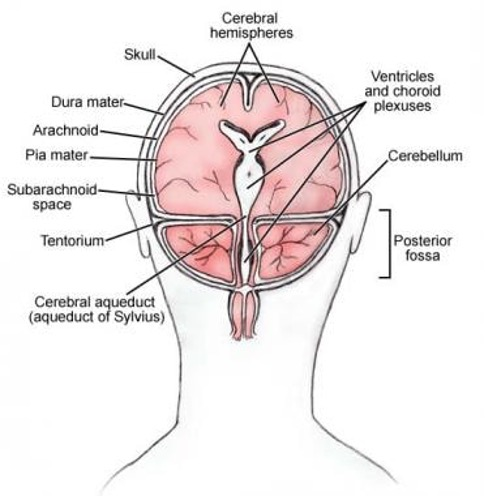
\includegraphics[width=0.5\linewidth,height=0.5\textheight,style="float:right; padding:10px"]{images/fig1}

\begin{itemize}
\item
  There is evidence to indicate that dynamic changes of specific brain
  regions over time may be likely associated with AD progression.
\item
  For example, subjects with MCI to AD conversion appear to be
  associated with increasingly enlarged ventricles across time, whereas
  subjects who did not progress to AD remained nearly unchanged.
\end{itemize}
\end{frame}

\begin{frame}{Research Objectives}
\protect\hypertarget{research-objectives}{}
\begin{itemize}
\item
  Investigate the association between the longitudinal feature of MRI
  images and time to AD.
\item
  Develop a prognostic model for clinicians to plan interventions based
  on the history of patients' MRI images.
\end{itemize}
\end{frame}

\begin{frame}{Data}
\protect\hypertarget{data}{}
\begin{itemize}
\item
  Alzheimer's Disease Neuroimaging Initiative (ADNI) study

  \begin{itemize}
  \tightlist
  \item
    Overall objective of detecting AD at the earliest stage and
    identifying ways to track the disease progression.
  \end{itemize}
\item
  Recruited subjects aged 55 to 90 and collected their imaging, genetic,
  clinical, cognitive, and biochemical characteristics across the
  long-term study.
\item
  Subjects could develop AD during the study period, so time-to-AD
  information was also collected.
\end{itemize}
\end{frame}

\begin{frame}{MRI Data}
\protect\hypertarget{mri-data}{}
\begin{itemize}
\item
  The preprocessed magnetic resonance imaging (MRI) data were obtained
  for each participant at several time points.
\item
  The image data for a given individual at a given time point can be
  stored in a voxel (i.e., 3D array structure) of dimension
  \(p= p_1 \times p_2 \times p_3\)
\item
  Voxel dimensions are the same across subjects and visits.
\item
  Images are voxel-wise stored, i.e., unfolded into a \(p\times1\)
  vector containing the voxels in a particular order, where the order is
  preserved across all subjects and visits.
\end{itemize}
\end{frame}

\begin{frame}{Complexities}
\protect\hypertarget{complexities}{}
\begin{itemize}
\tightlist
\item
  \textbf{Joint modeling}

  \begin{itemize}
  \tightlist
  \item
    Need model that incorporates dynamic variations/changing patterns of
    brain MRI images over time along with time-to-AD event information.
  \end{itemize}
\item
  \textbf{Ultrahigh-dimensional images}

  \begin{itemize}
  \tightlist
  \item
    MRI images are of dimension 133 × 170 × 129, so \(p\)=2,916,690
  \item
    Current joint modeling approaches have not considered settings when
    the longitudinal observations are Ultrahigh-dimensional.
  \end{itemize}
\item
  \textbf{Conducting dynamic prediction}

  \begin{itemize}
  \tightlist
  \item
    Existing prediction procedures only accommodate longitudinal
    low-dimensional observations.
  \end{itemize}
\end{itemize}
\end{frame}

\begin{frame}{Joint Modeling}
\protect\hypertarget{joint-modeling}{}
\begin{itemize}
\tightlist
\item
  The general concept is rather simple:

  \begin{enumerate}
  \tightlist
  \item
    We have longitudinal data
  \item
    We have survival data
  \item
    We want to model them in a way that the models borrow information
    from one another
  \end{enumerate}
\item
  Longitudinal data can inform survival outcome

  \begin{itemize}
  \tightlist
  \item
    e.g.~Increasing size of ventricles and the time to AD
  \end{itemize}
\item
  Survival can inform longitudinal data by accounting for informative
  censoring

  \begin{itemize}
  \tightlist
  \item
    e.g.~Missed visits due to progression to AD or death likely provides
    information on potentially unobserved trajectories of changes in the
    ventricles
  \end{itemize}
\end{itemize}
\end{frame}

\begin{frame}{Survival Data Background}
\protect\hypertarget{survival-data-background}{}
\begin{itemize}
\tightlist
\item
  What makes survival data unique is \emph{Censoring}
\item
  \emph{Censoring} occurs when we do not observe a subject until they
  experience the event of interest

  \begin{itemize}
  \tightlist
  \item
    May occur due to study ending, death due to another cause, or
    unrelated circumstances
  \end{itemize}
\end{itemize}

\textbf{Notation:}

\begin{itemize}
\tightlist
\item
  Let \(T_i^*\) be the actual survival time, which may or may not be
  observed due to censoring

  \begin{itemize}
  \tightlist
  \item
    The reason for \(^*\) is to distingish this time from the
    measurement times in the longitudinal data
  \end{itemize}
\item
  Let \(C_i\) be the censoring time
\item
  Define \(R_i\) = \(min(T_i^*, C_i)\), we call this the \emph{observed
  time}
\item
  Finally, define \(\Delta_i = I(T_i^* \leq C_i)\) to be the indicator
  of if the event was observed or not
\end{itemize}
\end{frame}

\begin{frame}{Modeling Survival Data}
\protect\hypertarget{modeling-survival-data}{}
\begin{itemize}
\tightlist
\item
  As the name implies, survival data depends on the survival
  distribution (S(t))
\item
  However, usually, the surivial function is defined in terms of a
  hazard function
\item
  The hazard function represents the instantaneous failure rate at time
  \(t\).
\item
  More specifically, it is the probability that a subject will fail at
  time \(t\) given that \(T^* > t\)
\item
  \(h(t) = \lim_{\delta \rightarrow 0} \frac{P(t + \delta > T^* > t | T^* > t)}{\delta}\)
\item
  \(h(t)\) relates to \(S(t)\) by \(h(t) = \frac{f(t)}{S(t)}\) where
  \(f(t) = -\frac{d}{dt}S(t) =\frac{d}{dt}F(t)\).
\item
  The hazard is often modeled using the Cox PH model:
\end{itemize}

\[
h(t|x) = h_0(t)exp \Big[Z_i \gamma \Big]
\]

\begin{itemize}
\tightlist
\item
  Where \(x\) at this point is an arbitrary stand in to represent
  ``data''
\item
  The above included only constant covariates
\end{itemize}
\end{frame}

\begin{frame}{Time Dependent Covariates}
\protect\hypertarget{time-dependent-covariates}{}
\begin{itemize}
\tightlist
\item
  Consider the following extension:
\end{itemize}

\[
h(t|x) = h_0(t)exp \Big[\boldsymbol{X}_i(t)\boldsymbol{\beta} + Z_i \gamma \Big]
\]

\begin{itemize}
\tightlist
\item
  This indicates that \(\boldsymbol{X}\) may be time dependent
\item
  Purely used to align with how the notation is presented in the paper.
\item
  ``May'' is critical for this presentation, \(\boldsymbol{X}(t)\) is
  currently an abuse of notation
\end{itemize}
\end{frame}

\begin{frame}{Back to Longitudinal}
\protect\hypertarget{back-to-longitudinal}{}
\begin{itemize}
\tightlist
\item
  Now that we have an idea of the form of the survival model, how will
  we model the images?
\item
  Model \(Y_{ij}\) with a mixed effects model with a random intercept
  and slope
\item
  Measured at times \(t_{ij}\)
\end{itemize}

\[
Y_{ij} = \mu_i + X_{i0} + X_{i1}T_{ij} + W_{ij} \\
\]

\begin{itemize}
\tightlist
\item
  \(Y_{ij}\) is the value actually observed at time \(t_{ij}\)
\item
  \(X_{i0}\) is a random intercept, and \(X_{i1}\) a random slope
\item
  \(W_{ij}\) is random normal error representing individual-visit
  variation
\item
  Note that the terms in the model above can be generalized
\end{itemize}
\end{frame}

\begin{frame}{Extension to Imaging Data}
\protect\hypertarget{extension-to-imaging-data}{}
\begin{itemize}
\tightlist
\item
  First, let \(\mu_i = \mu\)
\end{itemize}

\[
Y_{ij} = \mu + X_{i0} + X_{i1}T_{ij} + W_{ij} \\
\]

\begin{itemize}
\tightlist
\item
  Then note that we can model each voxel at a given visit \(j\):
\end{itemize}

\[
Y_{ij}(v) = \mu(v) + X_{i0}(v) + X_{i1}(v)T_{ij} + W_{ij}(v) \\
\]

\begin{itemize}
\item
  This simple change in notion introduces a shift in the modeling
  framework, as this is now a functional mixed effects model
\item
  The details of the functional form will be covered later
\end{itemize}
\end{frame}

\begin{frame}{Combining Models: The Survival model}
\protect\hypertarget{combining-models-the-survival-model}{}
\begin{itemize}
\tightlist
\item
  Recall the form presented previously:
\end{itemize}

\[
h(t|x) = h_0(t)exp \Big[\boldsymbol{X}_i(t)\boldsymbol{\beta} + Z_i \gamma \Big]
\]

\begin{itemize}
\tightlist
\item
  We will leave the fixed covariates as is, however, we will include the
  \textbf{REs} from the longitudinal model above as time varying
  covariates
\item
  With that said, survival is a univariate outcome, and we have brain
  scan data that is of much higher dimension

  \begin{itemize}
  \tightlist
  \item
    Integrate over this information
  \end{itemize}
\end{itemize}

\[
h(t|X_{i0}(v), X_{i1}(v), \boldsymbol{Z}_i) = h_0(t) exp \Big[ \int_{V} \lbrace \beta_0(v)X_{i0}(v) + t\beta_1(v)X_{i1}(v)\rbrace dv + \gamma'Z_i \Big]
\]

\begin{itemize}
\tightlist
\item
  Henderson Et. Al. 2000 provides the a more general form of the joint
  model, for which this is a subset of
\end{itemize}
\end{frame}

\begin{frame}{The Likelihood}
\protect\hypertarget{the-likelihood}{}
\begin{itemize}
\tightlist
\item
  Okay, great, but how do we actually fit this model?
\item
  To solve this problem, we need a likelihood
\item
  Let \(\boldsymbol{\theta}\) be the vector containing all unknown
  parameters
\item
  Then the general form of our likelihood is:
\end{itemize}

\[
p(\boldsymbol{R}, \boldsymbol{\Delta}, \tilde{\boldsymbol{Y}}, \boldsymbol{Z} | \boldsymbol{\theta})= \prod_{i=1}^I \int p(R_i, \Delta_i | \boldsymbol{X}_i(v), \boldsymbol{Z}_i, \boldsymbol{\theta})p(\boldsymbol{Y}_i|\boldsymbol{X}_i(v), \boldsymbol{\theta})p(\boldsymbol{X}_i(v)|\boldsymbol{\theta})d\boldsymbol{X}_i(v) 
\]

\begin{itemize}
\tightlist
\item
  In general, the arrival at a likelihood is not trivial
\item
  Tsiatis and Davidian (2004) covers the formulation of the likelihood
  which depends on the data itself and the modeling assumptions
\item
  Due to the treatment of high dimensional data, the likelihood here (to
  be presented), can be expressed in a form similar to that above, but
  does not have an explicit form
\end{itemize}
\end{frame}

\begin{frame}{PCA and Image Dimension Reduction - Basic Idea}
\protect\hypertarget{pca-and-image-dimension-reduction---basic-idea}{}
\begin{itemize}
\tightlist
\item
  The main idea is to use PCA to obtain low rank approximations of
  images.
\end{itemize}

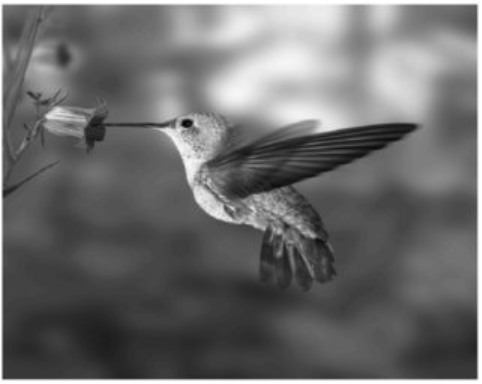
\includegraphics[width=0.5\linewidth,style="float:right; padding:20px"]{images/fig2a}

\begin{itemize}
\tightlist
\item
  Take for example this image:

  \begin{itemize}
  \tightlist
  \item
    This gray scale image is a 648 \(\times\) 600 image (i.e., p =
    388,800)
  \end{itemize}
\end{itemize}
\end{frame}

\begin{frame}{PCA and Image Dimension Reduction - Basic Idea}
\protect\hypertarget{pca-and-image-dimension-reduction---basic-idea-1}{}
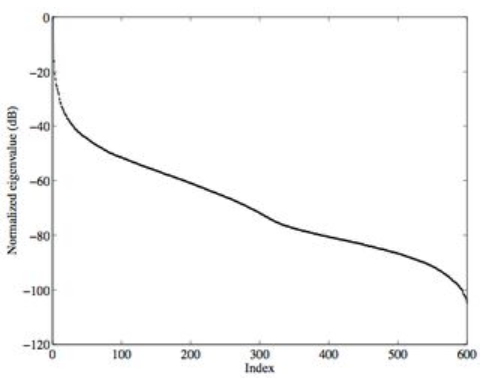
\includegraphics[width=0.4\linewidth,style="float:right; padding:20px"]{images/fig2b}

\begin{itemize}
\item
  Implement PCA using singular value decomposition (SVD).
\item
  Plot normalized eigenvalue by singular value (in this case there are
  600 total singular values).
\item
  After about the first 20−25 singular values, it falls off and the bulk
  of it is so low, that any information it contains is negligible.
\end{itemize}
\end{frame}

\begin{frame}{PCA and Image Dimension Reduction - Basic Idea}
\protect\hypertarget{pca-and-image-dimension-reduction---basic-idea-2}{}
\begin{itemize}
\tightlist
\item
  Image recreated by using the first 10 singular values (left) vs.~first
  50 (right)
\item
  Essence of the image is basically captured in just 10 singular values
  out of a total of 600.
\item
  Increasing to the first 50 singular values shows that the picture is
  almost exactly reproduced (to the human eye). Furthermore, only using
  the first 50 singular values essentially cuts down the dimensions of
  the original image by 84\%, while still preserving almost all the
  information from the original image.
\end{itemize}

\begin{center}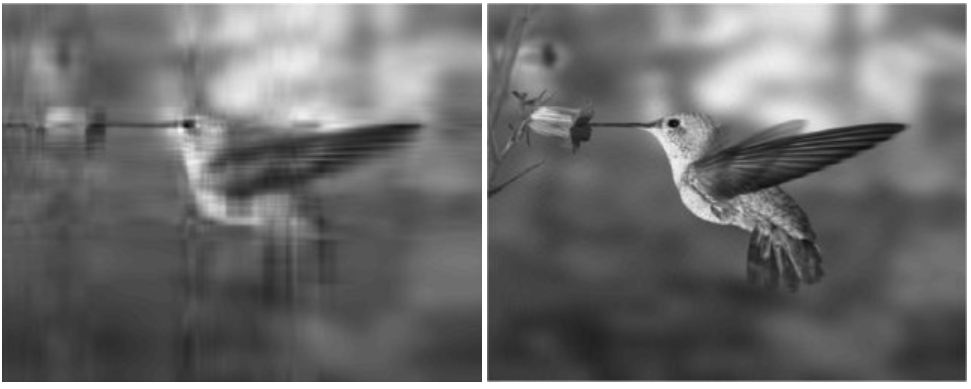
\includegraphics[width=0.7\linewidth]{images/fig2c} \end{center}
\end{frame}

\begin{frame}{PCA and Image Dimension Reduction - Basic Idea}
\protect\hypertarget{pca-and-image-dimension-reduction---basic-idea-3}{}
\begin{itemize}
\tightlist
\item
  Looking at the next 100 singular values (left), we see some fine
  structure, especially around the feathers, which are generally
  indistinguishable to the naked eye.
\item
  The smallest 300 singular values (right) convey no real information,
  most likely just noise.
\end{itemize}

\begin{center}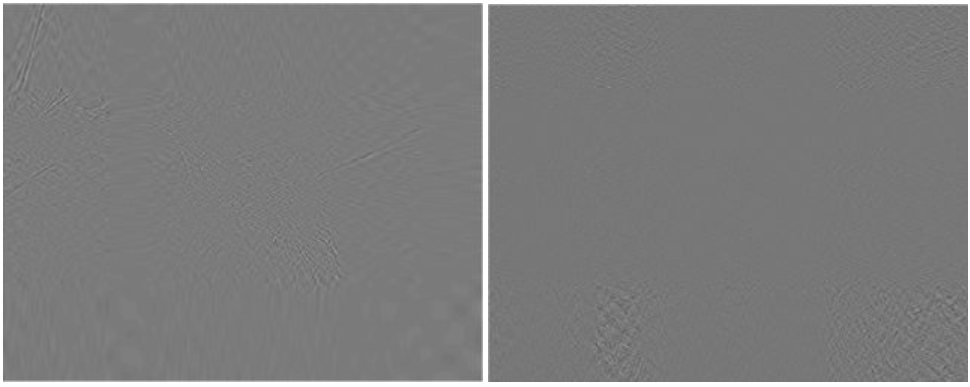
\includegraphics[width=0.7\linewidth]{images/fig2d} \end{center}
\end{frame}

\begin{frame}{KL Decomposition}
\protect\hypertarget{kl-decomposition}{}
\begin{itemize}
\item
  Let
  \(\mathrm{\bf{K}}^{X0}(v_1, v_2), \mathrm{\bf{K}}^{X1}(v_1, v_2), \text{ and } \mathrm{\bf{K}}^{W}(v_1, v_2)\)
  denote the covariance operator of \(X_{i0}(v), X_{i1}(v)\), and
  \(W_{ij}(v)\), respectively.
\item
  Based on KL decomposition, we have:

  \begin{itemize}
  \tightlist
  \item
    \(X_{i0}(v) = \sum^{\infty}_{k=1} \xi_{ik} \psi_{k}^{X0}(v)\)
  \item
    \(X_{i1}(v) = \sum^{\infty}_{l=1} \zeta_{il} \psi_{l}^{X1}(v)\)
  \item
    \(W_{ij}(v) = \sum^{\infty}_{m=1} \eta_{ijm} \psi_{m}^{W}(v)\)
  \end{itemize}
\item
  Where, \(\psi_{k}^{X0}(.), \psi_{l}^{X1}(.),\) and \(\psi_{m}^{W}(.)\)
  are the eigenfunctions of
  \(\mathrm{\bf{K}}^{X0}, \mathrm{\bf{K}}^{X1}\), and
  \(\mathrm{\bf{K}}^{W}\), respectively. Additionally,
  \(\xi_{ik}, \zeta_{il},\) and \(\eta_{ijm}\) are their corresponding
  eigenscores with:

  \begin{itemize}
  \tightlist
  \item
    \(E(\xi_{ik}) = E(\zeta_{il}) = E(\eta_{ijm}) = 0\)
  \item
    \(Var(\xi_{ik}) = \lambda_k^{X0}\)
  \item
    \(Var(\zeta_{il}) = \lambda_l^{X1}\)
  \item
    \(Var(\eta_{ijm}) = \lambda_m^{W}\)
  \end{itemize}
\end{itemize}
\end{frame}

\begin{frame}{KL Decomposition}
\protect\hypertarget{kl-decomposition-1}{}
Recall the longitudinal model described earlier:

\[
Y_{ij}(v) = \mu(v) + X_{i0}(v) + X_{i1}(v)T_{ij} + W_{ij}(v) \\
\]

Now it can be rewritten as

\[
Y_{ij}(v)=\mu(v) +\sum^{\infty}_{k=1} \xi_{ik} \psi_{k}^{X0}(v) + T_{ij}\sum^{\infty}_{l=1} \zeta_{il} \psi_{l}^{X1}+\sum^{\infty}_{m=1} \eta_{ijm} \psi_{m}^{W}(v) \\
\]

The model above can be approximated by the first few coordinates (i.e.,
principal components) (i.e., \(N_0 , N_1,\) and \(N_W\)) that are
typically small and determined using criterion-based methods (e.g.~BIC).
Giving us the eigenimages (i.e., low rank approximations of images).

\[
Y_{ij}(v)=\mu(v) +\sum^{N_0}_{k=1} \xi_{ik} \psi_{k}^{X0}(v) + T_{ij}\sum^{N_1}_{l=1} \zeta_{il} \psi_{l}^{X1}+\sum^{N_W}_{m=1} \eta_{ijm} \psi_{m}^{W}(v) \\
\]

\begin{itemize}
\tightlist
\item
  Where the eigenscores are assumed to be normally distributed as
  \(\xi_{ik} \sim N(0,\lambda_K^{X0})\),
  \(\zeta_{il} \sim N(0,\lambda_l^{X1})\), and
  \(\eta_{ijm} \sim N(0,\lambda_m^{W})\)
\end{itemize}

(Note: the normality assumption on the prior distributions of the
eigenscores can be relaxed without difficulty. Other distributions with
the existence of second order moments can be considered.)
\end{frame}

\begin{frame}{KL Decomposition}
\protect\hypertarget{kl-decomposition-2}{}
Recall the Cox model described earlier:

\[
h(t|X_{i0}(v), X_{i1}(v), \boldsymbol{Z}_i) = h_0(t) \exp \Big[ \int_{V} \lbrace \beta_0(v)X_{i0}(v) + t\beta_1(v)X_{i1}(v)\rbrace dv + \boldsymbol{\gamma}^\prime\boldsymbol{Z}_i  \Big]
\] Suppose \(\beta_0(v)\) and \(\beta_1(v)\) can be expanded on the
respective eigenfunctions \(\psi_k^{X0}\) and \(\psi_l^{X1}\), then
\(\beta_0(.)\) and \(\beta_1(.)\) can also be approximated by
\(\sum^{N_0}_{k=1}\beta_{0k}\psi_k^{X0}(v)\) and
\(\sum^{N_1}_{l=1}\beta_{1l}\psi_l^{X1}(v)\). This gives us the proposed
model:

\[
\begin{aligned}
h(t&|X_{i0}(v), X_{i1}(v), \boldsymbol{Z}_i) \\&= h_0(t) \exp \Big(\sum^{N_0}_{k=1}\beta_{0k}\xi_{ik}(v) + t\sum^{N_0}_{l=1}\beta_{1l}\zeta_{il}+\boldsymbol{\gamma}^\prime \boldsymbol{Z}_i  \Big)\\
&= h_0(t) \exp \Big(\boldsymbol{\beta}_0^\prime \boldsymbol{\xi}_i + t\boldsymbol{\beta}_1^\prime \boldsymbol{\zeta}_i+\boldsymbol{\gamma}^\prime \boldsymbol{Z}_i \Big)
\end{aligned}
\]

where \(\boldsymbol{\beta}_0 = (\beta_{01},...,\beta_{0N_0})^\prime\),
\(\boldsymbol{\xi}_i = (\xi_{i1},...,\xi_{iN_0})^\prime\),
\(\boldsymbol{\beta}_1 = (\beta_{11},...,\beta_{1N_1})^\prime\), and
\(\boldsymbol{\zeta}_i = (\zeta_{i1},...,\zeta_{iN_1})^\prime\)
\end{frame}

\begin{frame}{KL Decomposition - General Idea}
\protect\hypertarget{kl-decomposition---general-idea}{}
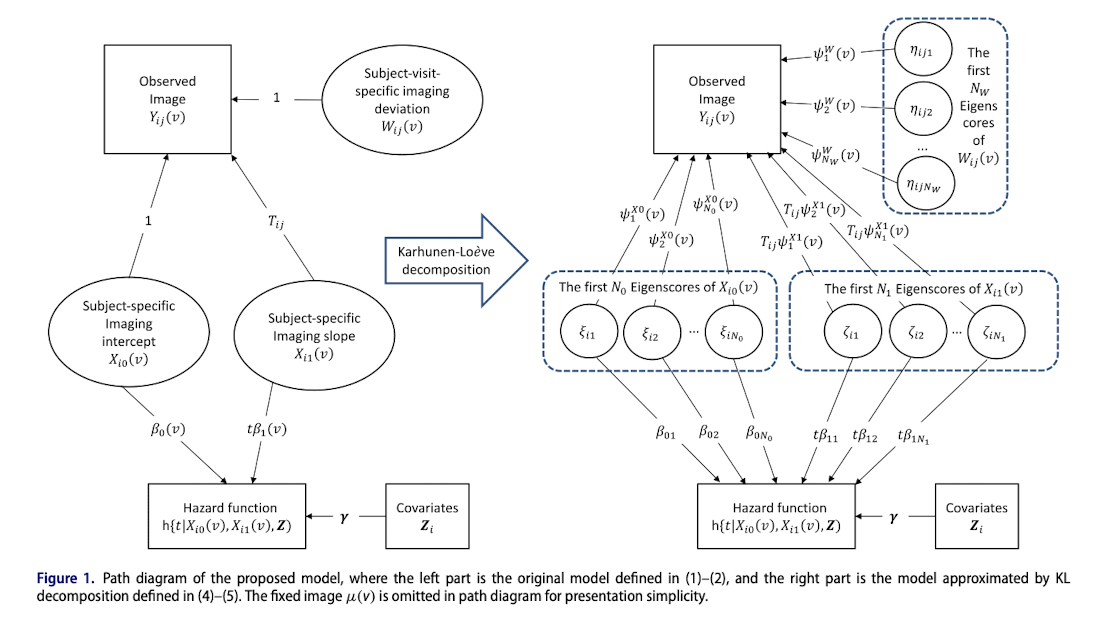
\includegraphics[width=0.85\linewidth,height=0.85\textheight,style="float:center; padding:10px"]{images/fig3}
\end{frame}

\begin{frame}{The Likelihood}
\protect\hypertarget{the-likelihood-1}{}
\begin{itemize}
\tightlist
\item
  Let
  \(\boldsymbol{D} = \lbrace \boldsymbol{R}, \boldsymbol{\Delta}, \tilde{\boldsymbol{Y}}, \boldsymbol{Z} \rbrace\)
\item
  Note that
  \(\boldsymbol{\theta} = \lbrace \boldsymbol{\beta}_0, \boldsymbol{\beta}_1, \boldsymbol{\gamma}, \boldsymbol{\lambda}_k^{X0}, \boldsymbol{\lambda}_l^{X1}, \boldsymbol{\lambda}_m^{W}, \boldsymbol{h}_g \rbrace\)
\item
  This leads to one single likelihood that can be used for fitting the
  model
\end{itemize}

\[
p(\boldsymbol{D} | \boldsymbol{\theta})= \prod_{i=1}^I \int \int p(R_i, \Delta_i | \boldsymbol{\xi}_i, \boldsymbol{\zeta}_i, \boldsymbol{Z}_i, \boldsymbol{\theta})p(\boldsymbol{Y}_i|\boldsymbol{\xi}_i, \boldsymbol{\zeta}_i, \boldsymbol{\theta})p(\boldsymbol{\xi}_i|\boldsymbol{\theta})p(\boldsymbol{\zeta}_i|\boldsymbol{\theta})d\boldsymbol{\zeta}_i d\boldsymbol{\xi}_i
\]

\begin{itemize}
\tightlist
\item
  Which does not have an explicit form
\end{itemize}
\end{frame}

\begin{frame}{Estimation}
\protect\hypertarget{estimation}{}
\begin{itemize}
\tightlist
\item
  In general, the route of estimation largely depends on the data at
  hand and the end goal
\item
  One simple way to go about this is to use a two stage approach:

  \begin{enumerate}
  \tightlist
  \item
    Estimate the longitudinal model
  \item
    Use estimates from (1) in the survival model
  \end{enumerate}
\item
  However this has been shown to lead to considerable bias when
  measurement error in the longitudinal observations are large
\item
  Many approaches use an EM algorithm adapted to the specific
  forumlation of the joint model
\item
  Other approaches have went Bayesian and developed MCMC algorithms
\item
  Given the complexity of the problem being solved here, the authors
  adopted a Bayesian approach
\end{itemize}
\end{frame}

\begin{frame}{Bayesian Details: Priors}
\protect\hypertarget{bayesian-details-priors}{}
\textbf{Unknown Parameters:}

\[
\begin{aligned}
\boldsymbol{\beta}_0 \sim N(\boldsymbol{0}, \sigma^2_{\beta_0}I_{N_0}) \\
\boldsymbol{\beta}_1 \sim N(\boldsymbol{0}, \sigma^2_{\beta_1}I_{N_1}) \\
\boldsymbol{\gamma} \sim N(\boldsymbol{0}, \sigma^2_{\gamma}I_{q})
\end{aligned}
\]

\begin{itemize}
\tightlist
\item
  The \(\sigma^2\)s are taken to be large when prior knowledge is not
  available
\end{itemize}

\textbf{Variance Components:}

For \(k = 1, \ldots, N_0\), \(l = 1, \ldots, N_1\),
\(m = 1, \ldots, N_w\),

\[
\begin{aligned}
\lambda_k^{X0} \sim IG(a_k^{X0}, b_k^{X0}) \\
\lambda_l^{X1} \sim IG(a_l^{X1}, b_l^{X1}) \\
\lambda_m^{W} \sim IG(a_m^{W}, b_m^{W}) \\
\end{aligned}
\]

\begin{itemize}
\tightlist
\item
  Empirical Bayes can be used to help choose hyper parameters
\item
  For example: \(a_k^{X0} \leq 0.01\),
  \(b_k^{X0} \leq 0.01\tilde{\lambda}_k^{X0}\), where
  \(\tilde{\lambda}_k^{X0}\) is the EB estimator
\end{itemize}
\end{frame}

\begin{frame}{Bayesian Details: Priors (continued)}
\protect\hypertarget{bayesian-details-priors-continued}{}
\textbf{Hazard values:}

\begin{itemize}
\tightlist
\item
  Here the approach taken to estimate \(h_0(t)\) is to treat it as a
  piecewise constant.
\end{itemize}

For \(g = 1, \ldots, G\),

\[
h_g \sim Gamma(\alpha_{1g}, \alpha_{2g})
\]

\begin{itemize}
\tightlist
\item
  With \((\alpha_{1g}, \alpha_{2g})\) often set to \((0.2, 0.4)\) or
  \((0.5, 1)\) to result in a flat prior.
\end{itemize}
\end{frame}

\begin{frame}{Bayesian Details: Sampling}
\protect\hypertarget{bayesian-details-sampling}{}
\begin{itemize}
\tightlist
\item
  Sampling directly from the posterior is intractable, as one might
  imagine

  \begin{itemize}
  \tightlist
  \item
    Mainly due to the existence of the latent variables
    \(\boldsymbol{\xi}\) and \(\boldsymbol{\zeta}\)
  \item
    Instead sampling is done for
    \(p(\boldsymbol{\theta}, \boldsymbol{\xi}, \boldsymbol{\zeta} | \boldsymbol{D})\)
  \end{itemize}
\item
  \(\boldsymbol{\eta}_{ij}\) can automatically be updated:
  \(\boldsymbol{\eta}_{ij} = (\Psi^{W'}\Psi^{W})^{-1}\Psi^{W'}(\tilde{\boldsymbol{Y}}_{ij} - \Psi^{X0}\boldsymbol{\xi}_i - T_{ij}\Psi^{X1}\boldsymbol{\zeta}_i)\)
\item
  The full conditionals for \(\boldsymbol{\xi}_i\) and
  \(\boldsymbol{\zeta}_i\) (jointly) and \(\boldsymbol{\beta}_0\),
  \(\boldsymbol{\beta}_1\), and \(\boldsymbol{\gamma}\) (jointly) are a
  bit unwieldy and don't follow a known distribution.

  \begin{itemize}
  \tightlist
  \item
    Required Metropolis Hastings with a multivariate normal proposal

    \begin{itemize}
    \tightlist
    \item
      Mean at the current value of the parameters of interest
    \item
      Covariance proportional to the inverse of the fisher information
      of the posterior

      \begin{itemize}
      \tightlist
      \item
        Use a small variance parameter to tune acceptance rate to be
        approximately 35\%
      \end{itemize}
    \end{itemize}
  \end{itemize}
\item
  The variances of the eigenscores and \(h_g\) can be sampled from using
  Gibbs sampling

  \begin{itemize}
  \tightlist
  \item
    The full conditionals for the variances (\(\lambda_k^{X0}\),
    \(\lambda_l^{X1}\), \(\lambda_m^{W}\)) are Inverse-Gamma
  \item
    The full conditionals for \(h_g\)s are Gamma
  \end{itemize}
\item
  Thus, Metropolis-Hastings within Gibbs can be used to sample from
  \(p(\boldsymbol{\theta}, \boldsymbol{\xi}, \boldsymbol{\zeta} | \boldsymbol{D})\)
\end{itemize}
\end{frame}

\begin{frame}{Bayesian Details: Prediction}
\protect\hypertarget{bayesian-details-prediction}{}
\begin{itemize}
\tightlist
\item
  Given a set of longitudinal images and baseline covariates we want to
  predict survival probability
\item
  Focus on the time interval \((t, t + \delta]\)
\item
  Conditional on surviving up to time \(t\), the conditional probability
  of survival up to time \(t +\delta\)
\item
  Notationally we are interested in
  \(P(T_i^* \geq t + \delta | T_i^* > t, Y_i^t, \boldsymbol{Z}_i, \boldsymbol{D})\)
\item
  Thus, we can compute the above probability with the integrand:
  \(\int P(T_i^* \geq t + \delta | T_i^* > t, Y_i^t, \boldsymbol{Z}_i, \boldsymbol{\theta})p(\boldsymbol{\theta}|\boldsymbol{D})d\boldsymbol{\theta}\)
\item
  The authors show this can be computed using Monte Carlo integration
\item
  Predictive ability can be assessed using a time dependent AUC

  \begin{itemize}
  \tightlist
  \item
    AUC(t, \(\delta\)) =
    \(P(\pi_{i_1}(t, \delta) < \pi_{i_2}(t, \delta) | \lbrace T^*_{i_1} \in (t, t + \delta] \rbrace \cap \lbrace T^*_{i_2} > t+ \delta \rbrace)\)
  \end{itemize}
\end{itemize}
\end{frame}

\begin{frame}{Data Analysis - Methods}
\protect\hypertarget{data-analysis---methods}{}
\begin{itemize}
\item
  Applied proposed method to ADNI dataset.
\item
  Only considered subjects who suffered from MCI at baseline and those
  with at least 3 longitudinal MRI scans: 339 subjects who had 3-6
  follow-up visits (baseline, month 6, month 12, month 18, month 24, and
  month 36).
\item
  127 subjects experienced conversion from MCI to AD.
\item
  Time to event was calculated as time from baseline to date of first
  diagnosis of AD for those that experience conversion and time from
  baseline to date of last visit for all others.
\item
  Censoring rate was approximately 62\%.
\item
  MRI data were preprocessed to a dimension of 133 × 170 × 129.
\item
  Considered demographic variables such as gender and whether or not the
  subject was married.
\item
  Considered the APOE gene biomarker. Included indicators for one APOE
  allele carrier and two APOE alleles carrier.
\end{itemize}
\end{frame}

\begin{frame}{Data Analysis - Methods}
\protect\hypertarget{data-analysis---methods-1}{}
\begin{itemize}
\item
  Used BIC to determine \(𝑁_0,𝑁_1,\) and \(𝑁_𝑤\) and assumed
  \(𝑁_0=𝑁_1=𝑁_𝑤=𝑁\). BIC selected \(𝑁=7\). Thus, the joint model with
  the first seven eigenimages was chosen for the analysis.
\item
  For the baseline hazard function they chose \(𝐺=5\) and selected the
  cut points as the quantiles of the observed survival time.
\item
  Used flat priors for the hyperparamters.
\item
  Used MCMC algorithm to collect 10,000 posterior samples after 10,000
  burn-in iterations.

  \begin{itemize}
  \tightlist
  \item
    5.03 minutes of computation time.
  \end{itemize}
\end{itemize}
\end{frame}

\begin{frame}{Data Analysis - Results}
\protect\hypertarget{data-analysis---results}{}
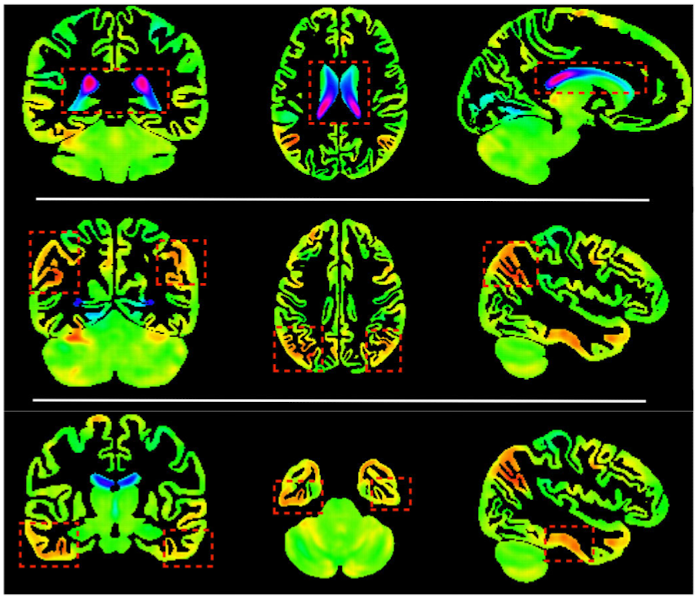
\includegraphics[width=0.3\linewidth,height=0.5\textheight,style="float:right; padding:10px"]{images/fig4}

\begin{itemize}
\tightlist
\item
  For the imaging predictors:

  \begin{itemize}
  \tightlist
  \item
    The 1st and 5th eigenimages of random imaging intercept and the 1st
    eigenimage of random imaging slope exhibit significant effects on AD
    hazards.
  \end{itemize}
\item
  Several brain regions are detected to be highly associated with AD
  hazards:

  \begin{itemize}
  \item
    The positive effect of ``lateral ventricles'' (the top row of
    figure) is evident, implying that the enlargement of the lateral
    ventricles is positively associated with the development of AD.
    Consistent with the previous medical studies.
  \item
    In the brain regions that depict negative effects, the magnitudes of
    the effects of ``inferior parietal lobe'' ( the second row of
    figure) and ``inferior temporal gyrus and fusiform gyrus'' (third
    row of figure) are relatively large. This is in line with existing
    research which indicate that AD is negatively correlated to the
    volume/thickness of these regions.
  \end{itemize}
\end{itemize}
\end{frame}

\begin{frame}{Data Analysis - Results}
\protect\hypertarget{data-analysis---results-1}{}
\begin{itemize}
\tightlist
\item
  For the baseline covariates:

  \begin{itemize}
  \tightlist
  \item
    Gender had a significant negative effect on AD hazards, indicating
    that females have a higher risk of suffering from AD than males.
  \item
    Surprisingly the APOE gene which has been found to be an important
    risk factor in previous research had an insignificant effect in this
    study.

    \begin{itemize}
    \tightlist
    \item
      One possible explanation is that APOE gene is somehow a
      confounding variable between certain brain regions and the hazards
      of AD.
    \end{itemize}
  \end{itemize}
\end{itemize}
\end{frame}

\begin{frame}{Questions}
\protect\hypertarget{questions}{}
\end{frame}

\begin{frame}{Spectral Decomposition}
\protect\hypertarget{spectral-decomposition}{}
\begin{itemize}
\item
  Spectral decomposition of
  \(\mathrm{\bf{K}}^{X0}, \mathrm{\bf{K}}^{X1}, \text{ and } \mathrm{\bf{K}}^{W}\)
  needs to be constructed to derive the eigenimages shown in the model.
\item
  Start by centering the longitudinal imaging data:

  \begin{itemize}
  \tightlist
  \item
    \(\tilde{Y}_{ij}(v) = Y_{ij}(v) - \hat{\mu(v)}\), where
    \(\hat{\mu(v)} = \frac{1}{n} \sum^I_{i=1} \sum^{J_i}_{j=1}Y_{ij}(v)\),
    \(n = \sum^I_{i=1}J_i\), \(I\) is the total number of subjects, and
    \(J_i\) is the total number of visits for subject i.
  \end{itemize}
\item
  However, we run into a problem due to \(\tilde{Y}_{ij}(v)\) being
  ultrahigh dimensional, making standard approaches for the spectral
  decomposition of
  \(\mathrm{\bf{K}}^{X0}, \mathrm{\bf{K}}^{X1}, \text{ and } \mathrm{\bf{K}}^{W}\)
  unfeasible.

  \begin{itemize}
  \tightlist
  \item
    For example, with the MRI images of 133 × 170 × 129 (
    \(p\)=2,916,690) the resulting covaraince operator
    \(\hat{\mathrm{\bf{K}}}^{X0}\) is of dimension 2,916,690 \(\times\)
    2,916,690.
  \end{itemize}
\item
  To overcome this challenge, use singular value decomposition (SVD):

  \begin{itemize}
  \tightlist
  \item
    Let
    \(\tilde{\mathrm{\bf{Y}}} = (\tilde{\mathrm{\bf{Y}}}_1, ..., \tilde{\mathrm{\bf{Y}}}_I)_{p \times n}\),
    where
    \(\tilde{\mathrm{\bf{Y}}}_i = (\tilde{\mathrm{\bf{Y}}}_{i1},...\tilde{\mathrm{\bf{Y}}}_{iJ_i})\)
    is the centralized \(p \times J_i\) and column \(j\) for
    \(j = 1,...,J_i\) contains the unfolded images for subject i at
    visit j
  \item
    Construct the singular value decomposition (SVD) of the matrix
    \(\tilde{\mathrm{\bf{Y}}}\) to get the best low-dimension
    approximation of the matrix which subsequently allows us to obtain a
    low-dimension representations of the covariance operator
    \(\hat{\mathrm{\bf{K}}}^{X0}, \hat{\mathrm{\bf{K}}}^{X1}, \text{ and } \hat{\mathrm{\bf{K}}}^{W}\).
  \end{itemize}
\end{itemize}
\end{frame}

\begin{frame}{Simulation Summary: Simulation 1 Setup}
\protect\hypertarget{simulation-summary-simulation-1-setup}{}
\begin{itemize}
\tightlist
\item
  Simulate 100 datasets with images of \(50 \times 50 \times 50\) and
  with \(\mu(v) = 0\).
\item
  In these simulations they use two different sample sizes: 300 and 500
\item
  Generate data with each subject having 7, 8, or 9 scans over time
\item
  Two principal components are used for the intercept and slope, and
  four are used for the random subject-visit deviation
\item
  They also considered three baseline hazards (constant, linear,
  non-linear) and a range of censoring rates
\item
  Evalutated Bias, RMSE, and SE
\end{itemize}
\end{frame}

\begin{frame}{Simulation Summary: Simulation 1 Results}
\protect\hypertarget{simulation-summary-simulation-1-results}{}
\begin{itemize}
\tightlist
\item
  Simulation 1 showed that the estimation procedure was satisfactory for
  estimating \(\boldsymbol{\beta}_0, \boldsymbol{\beta}_1\), and
  \(\boldsymbol{\gamma}\) as well as the estimates for the eigenscores.
\item
  They also found that performance is improved as the sample size is
  increased or censoring rate is decreased
\item
  Relatively consistent across different baseline hazards
\item
  Choice of \(N_W\) hardly effects estimation of survival model
\item
  Use of BIC to select \(N_0\) and \(N_1\), (where \(N_0\) = \(N_1\)),
  correctly selected 2 in 99 of the 100 simulations.
\item
  Each replication took about 4 and a half minutes.
\end{itemize}
\end{frame}

\begin{frame}{Simulation Summary: Simulation 2}
\protect\hypertarget{simulation-summary-simulation-2}{}
\begin{itemize}
\tightlist
\item
  Same setup as simulation 1, but focused on the comparison to the
  two-stage approach
\item
  Used a constant baseline hazard.
\item
  They also considered larger eigenscores for the subject-visit
  variation (1, 0.75, 0.5, 0.25)
\item
  Found that the two stage approach tends to produce biased results that
  does not improve with an increase in sample size

  \begin{itemize}
  \tightlist
  \item
    Worsens with an increase in the subject-visit variation as well
  \end{itemize}
\end{itemize}
\end{frame}

\end{document}
